\documentclass{ti2}

% Dateikodierung ist utf8
\usepackage[utf8]{inputenc}   
\usepackage{graphicx}
\usepackage{listings}
\usepackage{rotating}
\usepackage{nonfloat}

\usepackage{amsmath}

\lstset{
  numbers=left,
  numberstyle=\tiny,
  breaklines=true  
}

\begin{document}

% Nr, Abgabedatum, Gruppenleiter, Gruppenname, Name1...Name4
\Abgabeblatt{6}{12.12.2016}{Marc/Bingbin}{C05}%
                {Tabea Eggers}{Jan Fiedler}%
                {Florian Pflüger}{Jonas Schmutte}%

%\begin{listing}{1}
%\begin{listingcont}

\section*{Aufgabe 1}
Unsere mycp.cc befindet sich im Ornder ouraufgabe01.\\
Wir lassen die Main '-1' im Fehlerfall zur"ueckgeben.\\
\lstinputlisting[firstline=1,firstnumber=1,lastline=132]{ouraufgabe01/mycp.cc}
Ein Vergleich mit Ungerader Anzahl Bytes:\\
Es wurde vor jedem Kopieren der Cache gel"oscht.\\
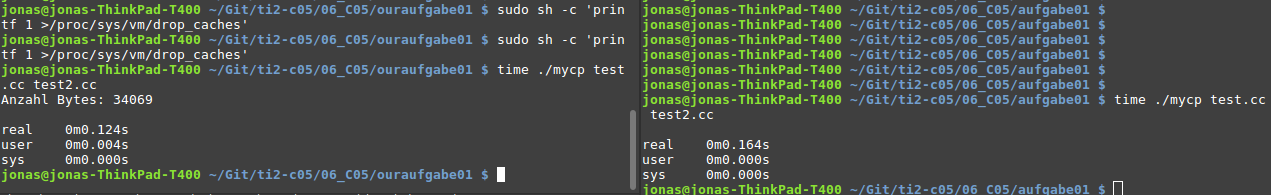
\includegraphics[width=\textwidth]{ouraufgabe01/testungeradebytes.png}
Das Ende der Datein danach (Der Rest stimmte auch "uberein):\\
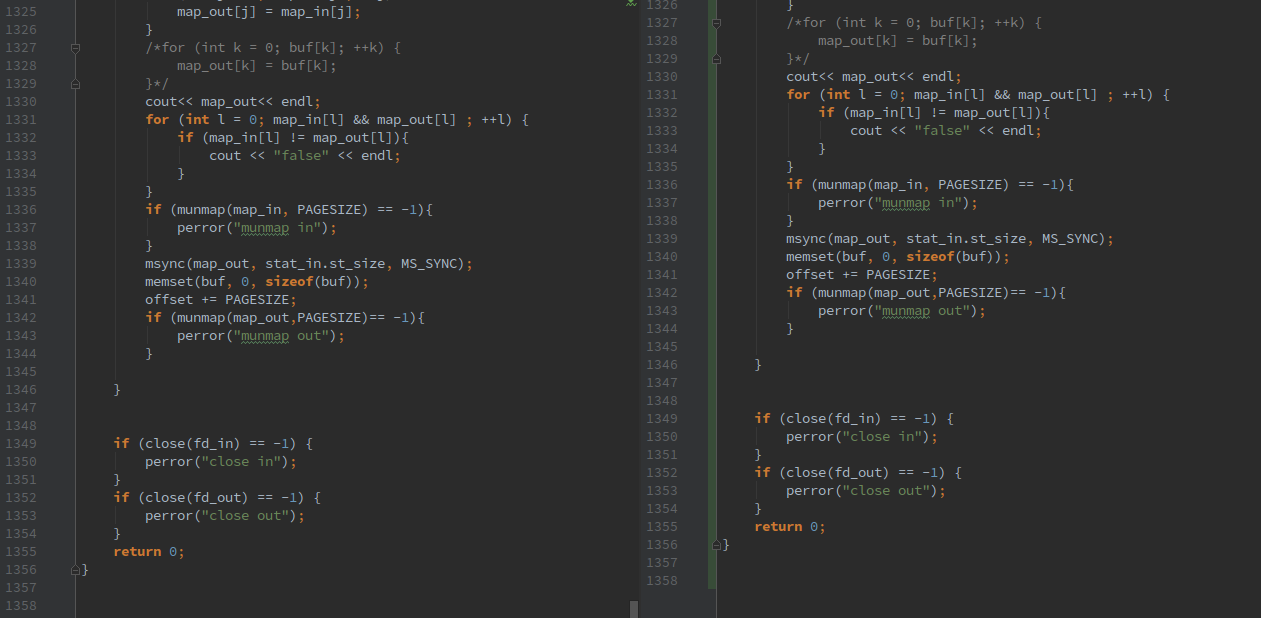
\includegraphics[width=\textwidth]{ouraufgabe01/vergleich.png}
Und die Tests f"ur Leere Datein.\\
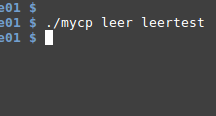
\includegraphics[width=\textwidth]{ouraufgabe01/leertest.png}
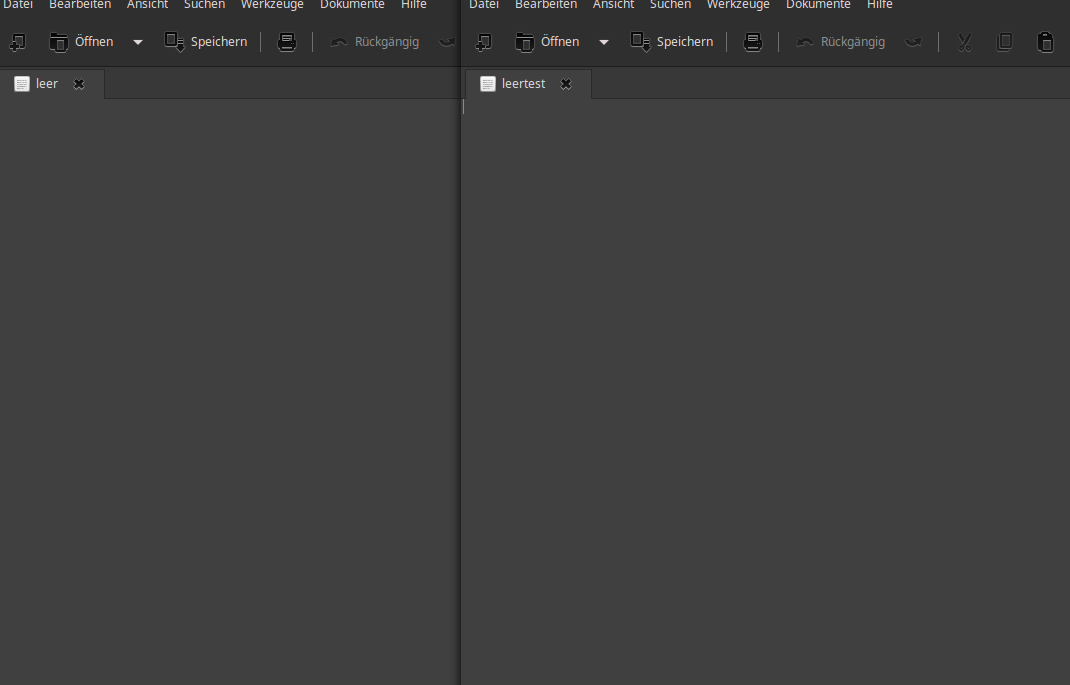
\includegraphics[width=\textwidth]{ouraufgabe01/leervergleich.png}

Bei uns haben auch andere Tests, das gleiche Verhalten gezeigt wie bei den hier gezeigten.\\
\section*{Aufgabe 2}
\textbf{gegeben:} \\
7200 Umdrehungen pro Minute \\
8 Oberflächen \\
100000 Spuren pro Oberfläche \\
1200 Sektoren pro Spur \\
512 Bytes pro Sektor \\
2,4 ms Kopfumschaltung beim Wechseln der Oberfläche \\
4 ms Spurenwechsel (inklusive möglicherweise erforderliche Kopfumstellung) \\
139586400 Byte Datei \\

\textbf{Berechnungen die für alle Aufgabenteile nützlich sind:}\\
\begin{align*}
\frac{139586400 B}{512 B} &= 272629 \text{Sektoren und } 352 B \Rightarrow \text{insgesamt 272630 Sektoren}\\
\frac{272630 \text{ Sektoren}}{1200 \text{ Sektoren pro Spur}} &= 227 \text{ volle Spuren und eine mit } 230 \text{ Sektoren} \Rightarrow 228 \text{ Spuren} \\
7200 \frac{\text{U}}{\text{min}} &= 120 \frac{\text{U}}{s} = 0,12 \frac{\text{U}}{\text{ms}} \Rightarrow 1 \text{ U} = \frac{25}{3} \text{ms} \approx 8,333 \text{ ms}\\
\end{align*}
\newcommand{\eu}{\frac{25}{3}\text{ms}}
\newcommand{\ms}{\text{ms}}

\textbf{a)}\\
Die bestmögliche Bedingung ist: das die Zylinder immer voll belegt sind und nur der letzte nicht voll belegt ist.
Somit wechselt man erst 7 mal die Oberfläche bevor man die Spur wechselt. \\
Berechnung: \\
\begin{align*}
\text{Die Datei braucht volle}&\text{ 227 Spuren und 230 Sektoren, also}\\
\frac{227 + 1}{8} &=  28 \text{volle Zylinder und } 4 \text{Oberfläche im 9 ten Zylinder.}\\
(28 + 1) \cdot 4 \ms + 28 \cdot 7 \cdot 2,4 \ms + 3 \cdot 2,4 \ms &= \frac{2968}{5} \ms = 593,6 ms \text{ für Oberflächen und Spuren wechsel}\\
\text{Nun die Zeit für die Umdrehungen:}\\
227 \cdot \eu + 230 \cdot \eu \cdot \frac{1}{1200} &= \frac{136315}{72} \ms = 1893,26388 \ms \text{für alle Sektoren}\\
\Rightarrow \text{Datenrate} &= \frac{139586560 B}{\frac{2968}{5} \ms + \frac{136315}{72} \ms} \approx 56129,55362 \frac{B}{\ms}\\
56129,55362 \frac{B}{\ms} \cdot \frac{1000}{1024} &\approx 54814,01721 \frac{\text{KiB}}{\text{s}} \approx 53,53 \frac{\text{MiB}}{\text{s}}
\end{align*}
\textbf{b)} \\
Die schlecht möglichste Bedingung ist: nach jedem Sektor muss die Spur gewechselt werden und weil der gesuchte Sektor dann gerade vorbei ist, muss noch eine Umdrehung lang gewartet werden. Also:\\
\begin{align*}
\frac{272630 \text{ Sektoren}}{100000 \text{Spuren}} &= 2 \text{ "{}volle"{} Oberfläche und eine dritte mit } 72630 \text{ Sektoren}\\
2 \cdot 100000 \cdot 4 \ms + 72630 \cdot 4 \ms &= 1090520 \ms \text{ für die Sprünge}\\
272630 \cdot \eu &= 2271917,667 \ms \\
\Rightarrow \text{ Datenrate:} \frac{13956560 B}{1090520 \ms + 2271917,667 \ms} &= \frac{1536}{37} \frac{B}{\ms}\\
&= \frac{1536}{37} \cdot \frac{1000}{1024} = \frac{1500}{37} \frac{KiB}{s} \approx 40,541 \frac{KiB}{s}
\end{align*}
\textbf{c)} \\
\begin{align*}
\intertext{Gleiche Verteilung wie in b) nun aber mit 4 KiB Blöcken}\\
\frac{272630 Sektoren}{8} &= 34079 \text{ Blöcke}\\
34079 \cdot \ms &= 136316 \ms \text{ für die Sprünge}\\
34079 \cdot \eu &= \frac{851975}{3} \ms \text{ fürs lesen}\\
\Rightarrow \text{Datenrate:} = \frac{34079 \cdot 8 \cdot 512 B}{136316 \ms + \frac{851975}{3}} &= 332,108 \frac{B}{\ms} = 324,324 \frac{KiB}{s}
\intertext{c ist also etwa 280 KiB/s  schneller als b}
\end{align*}

\section*{Aufgabe 3}
 $10000 Byte/s = 10Byte/ms$\\
 $1s = 1000ms$\\
 $1KiB = 1024B$

\textbf{a)}\\
Schreiben eines Byts dauert $0,1ms$. Dann brauchen wir inklusive auffüllen $0,1\frac{ms}{Byte} + 5ms = 5,1\frac{ms}{Byte}$. Somit hat dieses Gerät eine effektive Datenrate von 
\begin{align*}
	\frac{1000}{5,1\frac{ms}{Byte}}= 196,07843\frac{Byte}{s} \approx 196\frac{Byte}{s}
\end{align*}

\textbf{b)}\\
Effektives schreiben eines KiB dauert 
\begin{align*}
\frac{1024}{10\frac{Byte}{ms}} + 5ms = 107,4\frac{ms}{KiB}
\end{align*}
Somit hat dieses Gerät eine effektive Datenrate von
\begin{align*}
	\frac{1000}{107,4\frac{ms}{KiB}} \cdot 1024 = 9534,45065\frac{Byte}{s} \approx 9535\frac{Byte}{s}
\end{align*}

\textbf{c)}\\
Wir können von der effektiven Datenrate einfach die Zeit, die noch geschrieben wird während des erneuten Auffüllens, einfach abziehen, da dies ja parallel läuft.
\begin{align*}
	107,4\frac{ms}{KiB} - \frac{25ms}{10\frac{Byte}{ms}} = 104,9\frac{ms}{KiB}
\end{align*}
Somit hat dieses Gerät eine effektive Datenrate von
\begin{align*}
\frac{1000}{104,9\frac{ms}{KiB}} \cdot 1024 = 9761,67779\frac{Byte}{s} \approx 9762\frac{Byte}{s}
\end{align*}

\textbf{d)}\\
Formel umstellen:
\begin{align*}
	\frac{1000}{x} \cdot 1024 = 10000\\
	\frac{1000 \cdot 1024}{10000} = x = 102,4
\end{align*}
Somit müssen wir die Low-Watermark so hoch setzen, das ein KiB in $102,4ms$ abgearbeitet wird.
\begin{align*}
	107,4\frac{ms}{KiB} - 102,4\frac{ms}{KiB} = 5ms\\
	5ms \cdot 10\frac{Byte}{ms} = 50Byte
\end{align*}
Somit muss die Low-Watermark $50Byte$ betragen, damit die Netto-Datenrate des Geräts rechnerisch erreicht wird.
\end{document}
